\documentclass{article}
% For math environments
\usepackage{amsmath, amsfonts}
% For links
\usepackage[hidelinks]{hyperref}
% So space it put between paragraphs
\usepackage{parskip}
% For figures
\usepackage{tikz}
% Set the margins to not be ridiculous
\usepackage[margin=0.75in]{geometry}
% For multiple columns
\usepackage{multicol}
% For controlling enum/itemize spacing and indentation
\usepackage{enumitem}

% For tikz plots
\usepackage{pgfplots}
% This isn't needed but avoids a compiler warning
\pgfplotsset{compat=1.16}

% Allow multi-line equations to be broken across pages
\allowdisplaybreaks

% Use @ as a letter
\makeatletter

% Scale down all tikz coordinates while maintaining font size
\tikzset{every picture/.style={scale=0.45, every picture/.style={}}}


% Macros
% Monospace code
\def\code#1{\texttt{#1}}

% Greek letters
\def\a{\alpha}
\def\b{\beta}
\def\g{\gamma}
\def\d{\delta}
\def\D{\Delta}

% Some common sets
\def\es{\varnothing}
\def\ints{{\mathbb{Z}}}

% Commands that make life easier
\newcommand\gath[1]{\begin{gather} #1 \end{gather}}
\newcommand\gaths[1]{\begin{gather*} #1 \end{gather*}}
\newcommand\ali[1]{\begin{align} #1 \end{align}}
\newcommand\parens[1]{\left( #1 \right)}
\newcommand\squares[1]{\left[ #1 \right]}
\newcommand\braces[1]{\left\{ #1 \right\}}
\newcommand\angles[1]{\left\langle #1 \right\rangle}
\newcommand\deriv[2]{\frac{d #1}{d #2}}
\newcommand\abs[1]{\left| #1 \right|}
\newcommand\floor[1]{\left\lfloor #1 \right\rfloor}
\newcommand\ceil[1]{\left\lceil #1 \right\rceil}
\DeclareMathOperator{\lcm}{lcm}
\def\non{\nonumber \\}
\newcommand\unit[1]{~\mathrm{#1}}
\newcommand\combos[2]{{}_{#1}C_{#2}}

% Set stuff
\def\ss{\subseteq}

% Multiline equation space
\def\mlesp{\hspace{1.2cm}}

% For grid diagrams
\newcommand\gridbox[3]{\draw (#1,#2) rectangle (#1+1,#2+1) node[pos=.5] {#3};}
\newcommand\gridboxh[3]{\draw[fill=red!20] (#1,#2) rectangle (#1+1,#2+1) node[pos=.5] {#3};}
\newcommand\gridboxb[3]{\draw[fill=black] (#1,#2) rectangle (#1+1,#2+1) node[pos=.5] {#3};}
\newcommand\gridsym[3]{\node at (#1+0.5,#2+0.5) {$#3$};}
\newcommand\gridblank[2]{\filldraw[draw=gray, color=gray] (#1,#2) rectangle (#1+1,#2+1);}
\newcommand\gridcirc[2]{\draw (#1 + 0.5,#2 + 0.5) circle (0.25);}
\newcommand\cwlab[3]{
  \def\dd{0.15}
  \draw (#1 + \dd - 0.03, #2 + 1 - \dd) node {\scriptsize #3};
}

\def\bbw{3.5}
\def\bbh{2}
\newcommand\bigbox[3]{\draw (#1*\bbw,#2*\bbh) rectangle (#1*\bbw+\bbw,#2*\bbh+\bbh) node[pos=.5] {#3};}
\newcommand\bbtextr[3]{\node[right] at (#1*\bbw,#2*\bbh+0.5*\bbh) {#3};}
\newcommand\bbtextb[3]{\node[align=center] at (#1*\bbw+0.5*\bbw,#2*\bbh+0.5*\bbh) {#3};}

% Box puzzle stock answer
\newcommand\boxans[1]{
  Logic was used to deduce the solution:

  #1

  This was verified using Python as well as shown to be unique with a brute force approach.
}

% Standard crossnumber grid
\newcommand\crossnumstd[9]{
  \begin{center}
    \begin{tikzpicture}[scale=2]
      \gridbox{0}{2}{#1}
      \gridbox{1}{2}{#2}
      \gridbox{2}{2}{#3}
      \gridbox{0}{1}{#4}
      \gridbox{1}{1}{#5}
      \gridbox{2}{1}{#6}
      \gridbox{0}{0}{#7}
      \gridbox{1}{0}{#8}
      \gridbox{2}{0}{#9}

      % Labels
      \cwlab{0}{2}{1}
      \cwlab{1}{2}{2}
      \cwlab{2}{2}{3}
      \cwlab{0}{1}{4}
      \cwlab{0}{0}{5}
    \end{tikzpicture}
  \end{center}
}

% Multiple numbers
\newcommand\mn[1]{$#1$'s}

% Commands for problems
\newcommand\problem[4]{
\section*{#1}

\textbf{Question:} #3

\textbf{Answer:} #2

\textbf{Explanation:} #4
}
\newcommand\aproblem[4]{\problem{Dec #1}{#2}{#3}{#4}}
\newcommand\cproblem[4]{\problem{Problem #1}{#2}{#3}{#4}}

\newcommand\xref@advent[2]{#1 Advent, Dec~#2 problem}
\newcommand\xref@card[2]{#1 Christmas Card, Problem #2}

% For answered verified with Python
\newcommand{\verified}{This was verified with a brute-force Python program.}

\def\advent@xxi@i{
  The geometric mean of a set of $n$ numbers can be computed by multiplying together all the numbers then computing the $n$th root of the result.

  The factors of $4$ are $1$, $2$ and $4$. The geometric mean of these is 2.

  The factors of $6$ are $1$, $2$, $3$, and $6$. The geometric mean of these is $\sqrt{6}$.

  The geometric mean of all the factors of today's number is $22$.
}

\def\advent@xxi@ii{
  The number $7n$ has $37$ factors (including $1$ and the number itself).
  How many factors does $8n$ have?
}

\def\advent@xxi@iii{
  If you write out the numbers from $1$ to $1000$ (inclusive), how many times will you write the digit $0$?
}

\def\advent@xxi@iv{
  Put the digits $1$ to $9$ (using each digit exactly once) in the boxes so that the sums are correct.
  The sums should be read left to right and top to bottom ignoring the usual order of operations.
  For example, $4 + 3 \times 2$ is $14$, not $10$.
  Today's number is the product of the numbers in the red boxes.

  \grid@advent@xxi@iv{}{}{}{}{}{}{}{}{}
}

\def\advent@xxi@v{
  How many different isosceles triangles are there whose perimeter is $50$ units, and whose area is an integer number of units squared?

  (Two triangles that are rotations, reflections and translations of each other are counted as the same triangle. Triangles with an area of 0 should not be counted.)
}

\def\advent@xxi@vi{
  When $12345$ is divided by today's number, the remainder is $205$.
  When $6789$ is divided by today's number, the remainder is $112$.
}

\newcommand\dec@ai{0.30901699437494745}
\newcommand\dec@aii{0.8090169943749475}
\newcommand\dec@bi{0.5877852522924731}
\newcommand\dec@bii{0.9510565162951535}
\newcommand\decagon[5]{
  \def\ai{\dec@ai*#3+#1}
  \def\aii{\dec@aii*#3+#1}
  \def\bi{\dec@bi*#3+#2}
  \def\bii{\dec@bii*#3+#2}
  \draw (#3+#1, #2) -- (\aii, \bi) -- (\ai, \bii) -- (-\ai, \bii) -- (-\aii, \bi) -- (-#3+#1, #2) -- (-\aii, -\bi) -- (-\ai, -\bii) -- (\ai, -\bii) -- (\aii, -\bi) -- cycle;
  \fill[fill=red] (-\ai, -\bii) -- (#4*#3+#1, #5*#3+#2) -- (\ai, -\bii) -- cycle;
}
\def\advent@xxi@vii{
  The picture below shows eight regular decagons.
  In each decagon, a red triangle has been drawn with vertices at three of the vertices of the decagon.

  \begin{center}
    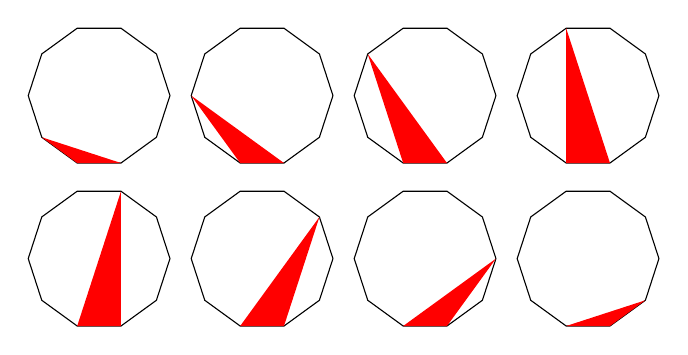
\begin{tikzpicture}
      \def\dr{2}
      \def\spc{2.3*\dr}

      \decagon{0*\spc}{\spc}{\dr}{-\dec@aii}{-\dec@bi}
      \decagon{1*\spc}{\spc}{\dr}{-1}{0}
      \decagon{2*\spc}{\spc}{\dr}{-\dec@aii}{\dec@bi}
      \decagon{3*\spc}{\spc}{\dr}{-\dec@ai}{\dec@bii}

      \decagon{0*\spc}{0}{\dr}{\dec@ai}{\dec@bii}
      \decagon{1*\spc}{0}{\dr}{\dec@aii}{\dec@bi}
      \decagon{2*\spc}{0}{\dr}{1}{0}
      \decagon{3*\spc}{0}{\dr}{\dec@aii}{-\dec@bi}
    \end{tikzpicture}
  \end{center}

  The area of each decagon is $240$.
  What is the total area of all the red triangles?
}

\def\advent@xxi@viii{
  The sum of three integers is $51$.
  The product of the same three integers is $836$. What is the product of largest integer and the second-largest integer?
}

\def\advent@xxi@ix{
  Eve writes down a sequence of consecutive positive integers (she writes more than one number).
  The sum of the numbers Eve has written down is $844$.
  Today's number is the smallest integer that Eve has written down.
}

\def\advent@xxi@x{
  Put the digits $1$ to $9$ (using each digit exactly once) in the boxes so that the sums are correct.
  Today's number is the largest number you can make using the digits in the red boxes.

  \grid@advent@xxi@x{}{}{}{}{}{}{}{}{}
}

\def\advent@xxi@xi{
  The integers are written in a triangle as shown below:
  \begin{center}
    \begin{tabular}{ccccccc}
         &    &    & 1    &    &    &    \\
         &    & 2  & 3    & 4  &    &    \\
         & 5  & 6  & 7    & 8  & 9  &    \\
      10 & 11 & 12 & 13   & 14 & 15 & 16 \\
         &    &    & etc. &    &    &
    \end{tabular}
  \end{center}
  Today's number appears directly above the number $750$ in the triangle of integers.
}

\def\advent@xxi@abgrid{
  \begin{center}
    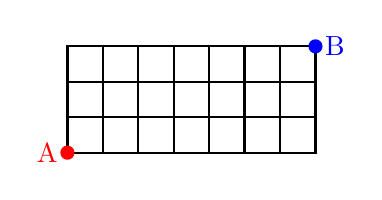
\begin{tikzpicture}
      \def\gs{1}
      % Grid
      \foreach \i in {0,...,6}{
          \foreach \j in {0,...,2}{
              \draw[thick] (\i * \gs, \j * \gs) rectangle (\i * \gs + \gs, \j * \gs + \gs);
            }
        }
      % Points
      \fill[color=red] (0, 0) circle (0.2) node[color=red,left] {A};
      \fill[color=blue] (7*\gs, 3*\gs) circle (0.2) node[color=blue,right] {B};
    \end{tikzpicture}
  \end{center}
}
\def\advent@xxi@xii{
  You start at the point marked A in the picture below. You want to get to the point marked B.
  You may travel \textbf{to the right} or \textbf{upwards} along the black lines.

  \advent@xxi@abgrid

  Today's number is the total number of possible routes to get from A to B.
}

\def\advent@xxi@xiii{
  The diagram below shows three circles and two triangles.
  The three circles all meet at one point.
  The vertices of the smaller red triangle are at the centers of the circles.
  The lines connecting the vertices of the larger blue triangle to the point where all three circles meet are diameters of the three circles.

  \begin{center}
    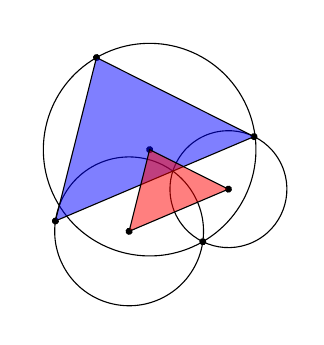
\begin{tikzpicture}[rotate=30,transform shape]
      \def\bcr{3}
      \def\scr{0.55*\bcr}
      \def\sca{34}
      \def\mcr{0.7*\bcr}
      \def\mca{142}
      \def\pr{0.1}

      % Circles
      \draw (0, \bcr) circle (\bcr);
      \draw (\sca: \scr) circle (\scr);
      \draw (\mca: \mcr) circle (\mcr);

      % Points
      \fill (0, 0) circle (\pr);
      \fill (0, \bcr) circle (\pr);
      \fill (0, 2*\bcr) circle (\pr);
      \fill (\sca: \scr) circle (\pr);
      \fill (\sca: 2*\scr) circle (\pr);
      \fill (\mca: \mcr) circle (\pr);
      \fill (\mca: 2*\mcr) circle (\pr);

      % Triangles
      \draw[fill=blue,fill opacity=0.5] (\mca: 2*\mcr) -- (0, 2*\bcr) -- (\sca: 2*\scr) -- cycle;
      \draw[fill=red,fill opacity=0.5] (\mca: \mcr) -- (0, \bcr) -- (\sca: \scr) -- cycle;
    \end{tikzpicture}
  \end{center}

  The area of the smaller red triangle is $226$.
  What is the area of the larger blue triangle?
}

\def\advent@xxi@xiv{
  You start at the point marked A in the picture below.
  You want to get to the point marked B.
  You may travel \textbf{to the right}, \textbf{upwards}, or \textbf{to the left} along the black lines, but you cannot pass along the same line segment more than once.

  \advent@xxi@abgrid

  Today's number is the total number of possible routes to get from A to B.
}

\newcommand\pyramid@advent@xxi@xvi[6]{
  \begin{center}
    \begin{tabular}{cccccc}
      (row 1) &    &    & #1   &    &    \\
      (row 2) &    & #2 &      & #3 &    \\
      (row 3) & #4 &    & #5   &    & #6 \\
              &    &    & etc. &    &
    \end{tabular}
  \end{center}
}
\def\advent@xxi@xv{
  The odd numbers are written in a pyramid.

  \pyramid@advent@xxi@xvi{1}{3}{5}{7}{9}{11}

  What is the mean of the numbers in the 19th row?
}

\newcommand\grid@advent@xxi@xvi[9]{
  \begin{center}
    \begin{tikzpicture}[scale=2]
      \gridbox{0}{2}{#1}
      \gridbox{1}{2}{#2}
      \gridbox{2}{2}{#3}
      \gridbox{0}{1}{#4}
      \gridbox{1}{1}{#5}
      \gridbox{2}{1}{#6}
      \gridbox{0}{0}{#7}
      \gridbox{1}{0}{#8}
      \gridbox{2}{0}{#9}

      % Labels
      \cwlab{0}{2}{1}
      \cwlab{1}{2}{2}
      \cwlab{2}{2}{3}
      \cwlab{0}{1}{4}
      \cwlab{0}{0}{5}
    \end{tikzpicture}
  \end{center}
}
\def\advent@xxi@xvi{
  Each clue in this crossnumber is formed of two parts connected by a logical connective: AND means that both parts are true; NAND means that at most one part is true; OR means that at least one part is true; NOR means that neither part is true; XOR means that exactly one part is true; XNOR means that either both parts are false or both parts are true.
  No number starts with $0$.

  \begin{multicols}{2}
    \grid@advent@xxi@xvi{}{}{}{}{}{}{}{}{}

    \columnbreak

    \begin{enumerate}
      \item \textbf{1A} is a palindrome XNOR \textbf{1D} is a palindrome.
      \item \textbf{1A} is greater than $350$ NOR \textbf{1D} is less than $150$.
      \item \textbf{3D} is odd NAND \textbf{4A} and \textbf{2D} are equal.
      \item \textbf{3D} is prime XOR \textbf{5A} is odd.
      \item \textbf{4A} is a cube AND \textbf{2D} is a cube.
      \item The sum of the digits of \textbf{3D} is $2$ OR the sum of the digits of \textbf{5A} is $5$.
      \item Today's number is \textbf{1D}.
    \end{enumerate}
  \end{multicols}
}

\def\advent@xxi@xvii{
  The digital product of a number is computed by multiplying together all of its digits. For example, the digital product of $6273$ is $252$.

  Today's number is the smallest number whose digital product is $252$.
}

\def\advent@xxi@xviii{
  Put the digits $1$ to $9$ (using each digit exactly once) in the boxes so that the sums are correct.
  The sums should be read left to right and top to bottom ignoring the usual order of operations.
  For example, $4 + 3 \times 2$ is $14$, not $10$.
  Today's number is the product of the numbers in the red boxes.

  \grid@advent@xxi@xviii{}{}{}{}{}{}{}{}{}
}

\def\advent@xxi@xix{
  The equation $352x^3 - 528x^2 + 90 = 0$ has three distinct real-valued solutions.

  Today's number is the number of integers $a$ such that the equation $352x^3 - 528x^2 + a = 0$ has three distinct real-valued solutions.
}

\def\advent@xxi@xx{
  What is the area of the largest area triangle that has one side of length $32$ and one side of length $19$?
}

\newcommand\grid@advent@xxi@xxi[9]{
  \begin{center}
    \begin{tikzpicture}
      \bigbox{0}{3}{#1}
      \bigbox{1}{3}{#2}
      \bigbox{2}{3}{#3}
      \bbtextr{3}{3}{\textbf{today's number}}

      \bigbox{0}{2}{#4}
      \bigbox{1}{2}{#5}
      \bigbox{2}{2}{#6}
      \bbtextr{3}{2}{prime}

      \bigbox{0}{1}{#7}
      \bigbox{1}{1}{#8}
      \bigbox{2}{1}{#9}
      \bbtextr{3}{1}{square}

      \bbtextb{0}{0}{cube}
      \bbtextb{1}{0}{odd}
      \bbtextb{2}{0}{multiple\\of $11$}
    \end{tikzpicture}
  \end{center}
}
\def\advent@xxi@xxi{
  Arrange the digits $1$–$9$ (using each digit exactly once) so that the three digit number in: the middle row is a prime number; the bottom row is a square number; the left column is a cube number; the middle column is an odd number; the right column is a multiple of $11$.
  The $3$-digit number in the first row is today's number.

  \grid@advent@xxi@xxi{}{}{}{}{}{}{}{}{}
}

\def\advent@xxi@xxii{
  There are $12$ ways of placing $2$ tokens on a $2 \times 4$ grid so that no two tokens are next to each other horizontally, vertically or diagonally:

  \begin{center}
    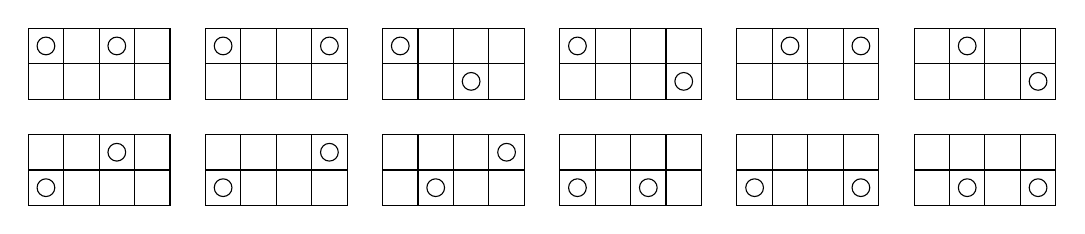
\begin{tikzpicture}
      % Draw all the grids
      \foreach \gi in {0,1}{
          \foreach \gj in {0,...,5}{
              \foreach \i in {0,1}{
                  \foreach \j in {0,...,3}{
                      \gridbox{5*\gj + \j}{3*\gi + \i}{}
                    }
                }
            }
        }

      % Place token circles
      \gridcirc{0}{4}
      \gridcirc{2}{4}
      \gridcirc{5}{4}
      \gridcirc{8}{4}
      \gridcirc{10}{4}
      \gridcirc{12}{3}
      \gridcirc{15}{4}
      \gridcirc{18}{3}
      \gridcirc{21}{4}
      \gridcirc{23}{4}
      \gridcirc{26}{4}
      \gridcirc{28}{3}
      \gridcirc{0}{0}
      \gridcirc{2}{1}
      \gridcirc{5}{0}
      \gridcirc{8}{1}
      \gridcirc{11}{0}
      \gridcirc{13}{1}
      \gridcirc{15}{0}
      \gridcirc{17}{0}
      \gridcirc{20}{0}
      \gridcirc{23}{0}
      \gridcirc{26}{0}
      \gridcirc{28}{0}
    \end{tikzpicture}
  \end{center}

  Today's number is the number of ways of placing $2$ tokens on a $2 \times 21$ grid so that no two tokens are next to each other horizontally, vertically or diagonally.
}

\def\advent@xxi@xxiii{
  I draw the parabola $y = x^2$ and mark points on the parabola at $x = 17$ and $x = -6$.
  I then draw a straight line connecting these two points.

  At which value of $y$ does this line intercept the $y$-axis?
}

\def\advent@xxi@xxiv{
  The digital product of a number is computed by multiplying together all of its digits.
  For example, the digital product of $1522$ is $20$.

  How many $12$-digit numbers are there whose digital product is $20$?
}

\def\card@xxi@i{
  What is the sum of all the odd integers between $0$ and $30$?
}

\def\card@xxi@ii{
  What is the sum of all the odd integers between $0$ and $5668$?
}

\def\card@xxi@iii{
  What is the smallest integer with a digital sum of $28$ and a digital product of $10000$?
}

\def\card@xxi@iv{
  What is the smallest integer with a digital sum of $41$ and a digital product of $432000$?
}

\def\card@xxi@v{
  What is the area of the largest area dodecagon that will fit inside a circle with area $111185 \pi$?
}

\def\card@xxi@vi{
  What is the area of the largest area heptagon that will fit inside a semicircle with area $115185 \pi$?
}

\def\card@xxi@vii{
  How many terms are there in the (simplified) expansion of $(x + y + z)^2$?
}

\def\card@xxi@viii{
  How many terms are there in the (simplified) expansion of $(x + y + z)^{41172}$?
}

\def\card@xxi@ix{
  What is the largest integer that cannot be written as $4a + 5b$ for non-negative integers $a$ and $b$?
}

\def\card@xxi@x{
  What is the largest integer that cannot be written as $83409a + 66608b$ for non-negative integers $a$ and $b$?
}

\def\card@xxi@xi{
  How many positive integers are there below $100$ whose digits are all non-zero and different?
}

\def\card@xxi@xii{
  How many positive integers are there whose digits are all non-zero and different?
}

\def\card@xxi@xiii{
  What is the only integer for which taking the geometric mean of all its factors (including $1$ and the number itself) gives $2$?
}

\def\card@xxi@xiv{
  What is the only integer for which taking the geometric mean of all its factors (including $1$ and the number itself) gives $25$?
}

\input{boxes}

\begin{document}

\title{MS Scroggs Advent Calendar 2019 Answers}
\author{Dan Whitman}
\date{}

\maketitle

Answers: \href{https://www.mscroggs.co.uk/puzzles/advent2019}{https://www.mscroggs.co.uk/puzzles/advent2019}

\aproblem{1}{301}{\advent@xix@i}{
  Each of the digits will be one 100 times since there are 100 combinations of the other two digits.
  Thus the total number of ones written in the numbers 1 to 999 are
  $$
  100 + 100 + 100 = 300 \,.
  $$
  Then of course 1000 only has one 1 so that the final answer is $300 + 1 = 301$.

  This answer was verified using Python.
}

\aproblem{2}{203}{\advent@xix@ii}{
  A valid triangle can only be formed when the sum of two sides is greater than the third side, so we really only need to check that the two smallest sides sum to greater than the third, largest side.
  If the sum is equal to the third side the sticks must “lay on top of each other,'' which we are told is not a valid triangle.
  Furthermore, given three valid sides, the triangle is unique up to reflection and rotation.
  A Python script was written to count the number of valid triangles for this set of sides, i.e. where the two shortest sides sum to greater than the longest side.
}

\aproblem{3}{432}{\advent@xix@iii}{
  \boxans{\gridsol@advent@xix@iii}
}

\newcommand\tilerect[2]{\draw[color=red!75,line width=2] (#1) rectangle (#2);}
\newcommand\tilefig[2]{
  \begin{tikzpicture}
    \draw (0,0) grid (#1);
    #2
  \end{tikzpicture}
  \qquad
}
\def\contd{
  \draw (0,0) -- (0,-0.5);
  \draw (1,0) -- (1,-0.5);
  \draw (2,0) -- (2,-0.5);
  \node[align=center] at (1,-0.7) {$\cdots$};
}

\aproblem{4}{341}{\advent@xix@iv}{
  There are clearly exactly 3 ways to tile a $2 \times 2$ grid:
  \begin{center}
    \tilefig{2,2}{
      \tilerect{0,0}{2,2}
    }
    \tilefig{2,2}{
      \tilerect{0,0}{1,2}
      \tilerect{1,0}{2,2}
    }
    \tilefig{2,2}{
      \tilerect{0,0}{2,1}
      \tilerect{0,1}{2,2}
    }
  \end{center}
  Let $s_n$ denote the the number of ways to tile an $n \times 2$ grid.
  Then we know that $s_1 = 1$ and $s_2 = 3$.
  We can generally determine $s_n$ using an approach similar to strong induction.
  If we know $s_k$ for $k < n$, then there are 3 ways to cover the first row of an $n \times 2$ grid:
  \begin{center}
    \tilefig{2,3}{
      \contd
      \tilerect{0,1}{2,3}
    }
    \tilefig{2,3}{
      \contd
      \tilerect{0,1}{1,3}
      \tilerect{1,1}{2,3}
    }
    \tilefig{2,3}{
      \contd
      \tilerect{0,2}{2,3}
    }
  \end{center}
  For each of the first two of these ways we must cover the remaining $(n-2) \times 2$ grid and there are of course $s_{n-2}$ ways to do this.
  For the third we must cover the remaining $(n-1) \times 2$ grid, of which there are $s_{n-1}$ ways.
  Therefore the total number of ways to cover an $n \times 2$ grid is
  $$
  s_n = s_{n-2} + s_{n-2} + s_{n-1} = s_{n-1} + 2s_{n-2} \,.
  $$
  This forms a sequence not unlike the Fibonacci sequence.
  The first ten elements of the sequence are:
  \begin{center}
    \begin{tabular}{c|cccccccccc}
      $n$ & 1 & 2 & 3 & 4 & 5 & 6 & 7 & 8 & 9 & 10 \\
      \hline
      $s_n$ & 1 & 3 & 5 & 11 & 21 & 43 & 85 & 171 & 341 & 683
    \end{tabular}
  \end{center}
  Thus the answer is $s_9 = 341$.
  This sequence was confirmed to be correct on OEIS, and is the Jacobsthal sequence.
  The notes for this sequence mention it being the number of ways to tile a $n \times 2$ grid using the specified dominoes.
}

\aproblem{5}{364}{\advent@xix@v}{
  The 28 points on the circle are spaced $\Delta \theta = 360/28 = 90/7 \approx 12.86$ degrees apart.
  The radius of the circle is of course irrelevant here so we may as well use the unit circle.
  We number the points $p_n$ for $0 \leq n < 28$ and we can place $p_0$ at $(1,0)$ and count counterclockwise so that we have the following example points that divide the circle into quarters:
  \begin{center}
    \begin{tabular}{c|c}
      $n$ & $p_n$ \\
      \hline
      0 & $(1,0)$ \\
      7 & $(0,1)$ \\
      14 & $(-1,0)$ \\
      21 & $(0,-1)$
    \end{tabular}
  \end{center}
  Now, given one of the 28 points as a base, say $p = p_{14} = (-1,0)$, we can choose any other 2 distinct points to create a triangle.
  However, clearly this triangle will be isosceles with the two equal sides emanating from $p$ only when a point on the top half is chosen along with its mirror point on the bottom half when reflected over the $x$-axis.
  As there are 13 of these point-pairs, 13 of the triangles emanating from $p$ will be isosceles.
  Since this is done for each of the 28 points, there can be at most $13 \cdot 28 = 364$ isosceles triangles.

  The question arises as to whether we are counting some isosceles triangles more than once though.
  The only way this could be the case is if we have equilateral triangles wherein more than one point acts as the base from which the equal sides emanate.
  However, a third of the circle or $360/3 = 120$ degrees is not an integer multiple of our $\Delta \theta$, which means that no 3 of our 28 points can be evenly spaced around the circle.
  Because of this there can be no equilateral triangles since sides of any triangle is the chord length $2\sin(\theta/2)$, where $\theta$ is the positive angle between the points.
  From this it follows that we have exactly $364$ isosceles triangles.

  This answer was confirmed with a brute force Python program.
}

\aproblem{6}{221}{\advent@xix@vi}{
  Suppose that Noel has $N$ grandchildren, and let $t_n$ be the total number of pounds given to all his grandchildren on the year that the \emph{youngest} is $n$ years old (and therefore gets $n$ pounds).
  As the children were all born on consecutive years, the total they are given on year $n$ is
  $$
  t_n = \sum_{i=0}^{N-1} (n+i) = \sum_{i=0}^{N-1} n + \sum_{i=0}^{N-1} i = Nn + \sum_{i=1}^{N-1} i = Nn + \frac{N(N-1)}{2} = \frac{N(N + 2n - 1)}{2} \,,
  $$
  noting that this is monotonically increasing in both $N$ and $n$.
  Python was used to evaluate $t_n$ for all combinations of $N,n \in \{1, 2, \ldots, 20\}$.
  It showed that the only combination where $t_n = 208$ is for $N = 13$ and $n = 10$.
  Note that, because of the monotonicity of $t_n$ in both $N$ and $n$, $t_n > 208$ for all $N > 13$ and $n > 10$ so that we a guaranteed not to have another combination where $t_n = 208$.
  Hence the total number of pounds his grandchildren get the next year is $t_{n+1} = t_n + N = 221$.
}

\aproblem{7}{243}{\advent@xix@vii}{
  In general, the binomial theorem states that
  $$
  (x+y)^n = \sum_{k=0}^n \binom{n}{k} x^{n-k} y^k \,,
  $$
  where of course $\binom{n}{k}$ are the binomial coefficients.
  Hence, for the example we have
  $$
  (x+1)^5 = (1+x)^5 = \sum_{k=0}^5 \binom{5}{k} 1^{5-k} x^k = \sum_{k=0}^5 \binom{5}{k} x^k
  $$
  so that the sum of coefficients is simply
  $$
  \sum_{k=0}^5 \binom{5}{k} = 32
  $$
  as confirmed using Python.
  For the main problem we then have
  $$
  (2x+1)^5 = (1+2x)^5 = \sum_{k=0}^5 \binom{5}{k} 1^{5-k} (2x)^k = \sum_{k=0}^5 \binom{5}{k} 2^k x^k \,,
  $$
  and thus the sum of the coefficients is
  $$
  \sum_{k=0}^5 \binom{5}{k} 2^k = 243
  $$
  as calculated in Python.
  This answer was also verified by expanding $(2x+1)^5$ in Wolfram Alpha and summing the $6$ coefficients manually.
}

\aproblem{8}{270}{\advent@xix@viii}{
  Generally we want the highest digits in the tens places and the lowest digits in the ones places, noting again that all five numbers must be even.
  However, it does not matter which ones digit goes with which number.
  For example
  \begin{align*}
    10 + 32 + 54 + 76 + 98 &= (10 + 0) + (30 + 2) + (50 + 4) + (70 + 6) + (90 + 8) \\
    &= (10 + 8) + (30 + 6) + (50 + 4) + (70 + 2) + (90 + 0) \\
    &= 18 + 36 + 54 + 72 + 90 \\
    &= 270 \,,
  \end{align*}
  which is in fact the largest possible sum.
  This was verified in Python using a brute force method to check every possible permutation of digits into 5 two-digit numbers.
}

\aproblem{9}{523}{\advent@xix@ix}{
  \boxans{\grid@advent@xix@ix{5}{7}{1}{2}{8}{4}{3}{9}{6}}
}

\aproblem{10}{256}{\advent@xix@x}{
  Define $g(x) = 8x - 8 - x^2$ and $h(x) = x^2$, which are of course both parabolas.
  Then we know that $g(x) \leq f(x) \leq h(x)$ for all real $x$.
  A plot of $g$ and $h$ are shown below:
  
  \newcommand\doplot[1]{
    \begin{center}
      \begin{tikzpicture}[scale=1.8]
        \begin{axis}[
            axis lines=middle,
            xmin=-5, xmax=5,
            ymin=-70, ymax=30,
            samples=100,
          ]
          \addplot[
            blue,
            thick,
            domain=-5:5,
          ]
          (x, x^2);
          \node [above right] at (axis cs:-4,16) {$h$};
          \addplot[
            red,
            thick,
            domain=-5:5,
          ]
          (x, 8*x - 8 - x^2);
          \node [below right] at (axis cs:-4,-56) {$g$};
          #1
        \end{axis}
      \end{tikzpicture}
    \end{center}
  }
  \doplot{}
  
  We notice that they appear to touch at a single point and that there seems to be just enough space for a single line to squeeze through.
  To see whether they touch at a single point we set
  \begin{gather*}
    g(x) = h(x) \\
    8x - 8 - x^2 = x^2 \\
    8x - 8 = 2x^2 \\
    4x - 4 = x^2 \\
    x^2 - 4x + 4 = 0 \\
    (x - 2)^2 = 0 \,.
  \end{gather*}
  Therefore they intersect at the single point $(2, g(x)) = (2, h(2)) = (2, 4)$.
  Hence we also must have $4 = g(2) \leq f(2) \leq h(2) = 4$ so that $f(2) = 4$.
  We also have that $g'(x) = 8 - 2x$ and $h'(x) = 2x$ so that $g'(2) = h'(2) = 4$.
  Indeed it must be that $g$ and $h$ have the same slope at their intersection point in order for a line to pass in between them at all points.

  So the line we seek is the tangent line of both parabolas at their intersection point.
  That is a line with slope $a = 4$ and passes through the point $(2,4)$.
  Solving $4 = f(2) = 4 \cdot 2 + b$ for $b$ results in our line $f(x) = 4x-4$.
  A plot of the parabolas along with this line is shown below:

  \doplot{
    \addplot[
      black,
      thick,
      domain=-5:5,
    ]
    (x, 4*x - 4);
    \node [below right] at (axis cs:-4,-20) {$f$};
  }
  
  This confirms that $f$ is the correct line.
  Therefore the answer is $f(65) = 256$.
}

\aproblem{11}{192}{\advent@xix@xi}{
  \boxans{\gridsol@advent@xix@xi}
}

\aproblem{12}{643}{\advent@xix@xii}{
  There are $T = 650 \cdot 99 = 64350$ total voters.
  Half of these voted for the Rum party, which is of course $T/2$, noting that this is an integer since $T$ is even.
  Now, the Rum party must get exactly $50$ votes in a district to win the MAP and ``spend'' the minimum number of its $T/2$ voters since this is a minimal majority for $99$ voters.
  Therefore the maximal number of MAPs that the Rum party can win is $\lfloor T/2/50 \rfloor = \lfloor T/100 \rfloor = 643$, noting that the floor is necessary since a district with less than $50$ votes will not be won.
}

\aproblem{13}{211}{\advent@xix@xiii}{
  \boxans{\grid@advent@xix@xiii{2}{1}{5}{2}{1}{2}{1}{1}{9}}
}

\aproblem{14}{112}{\advent@xix@xiv}{
  This was solved with a simple Python script that sums the digits and counts how many add to $14$.
}

\aproblem{15}{203}{\advent@xix@xv}{
  This was solved using Python, which was challenging to implement.
  It was noticed that both $30 = 2 \cdot 3 \cdot 5$ and $30030 = 2 \cdot 3 \cdot 5 \cdot 7 \cdot 11 \cdot 13$ factor into unique prime factors with no repeated factors.
  If $f(n)$ denotes the number of ways to multiply a number with $n$ unique prime factors, then this forms the following sequence, which was determined by experimentation with the Python script:
  \begin{center}
    \begin{tabular}{c|c}
      $n$ & $f(n)$ \\
      \hline
      1 & 1 \\
      2 & 2 \\
      3 & 5 \\
      4 & 15 \\
      5 & 52 \\
      6 & 203 \\
      7 & 877
    \end{tabular}
  \end{center}
  Looking it up on OEIS, this is the Bell sequence, given by the recurrence relation
  $$
  f(n) = \sum_{k=0}^n \binom{n}{k} f(k) \,.
  $$
  I struggled to deduce this relation but failed.
}

\aproblem{16}{921}{\advent@xix@xvi}{
  Tried to deduce the grid solution, but eventually got stuck and would have had to guess.
  As such, this was just solved using a brute force search in Python:

  \grid@advent@xix@xvi{9}{6}{5}{2}{8}{3}{1}{7}{4}
}

\aproblem{17}{193}{\advent@xix@xvii}{
  Let $x$ be Eve's original number with the digits $d_2 d_1 d_0$, and let $y$ be the second, reversed number, which would then have digits $d_0 d_1 d_2$.
  Now, we know that $d_2 > 0$ since $x$ is a three-digit number.
  We are also told that $y > x$, from which it follows that $d_2 \neq d_0$ since otherwise it would be that $x = y$.
  Moreover we must have $d_0 > d_2$ since $y > x$.
  Lastly, we know that
  \begin{gather*}
    x + y = 584 \\
    (100 d_2 + 10 d_1 + d_0) + (100 d_0 + 10 d_1 + d_2) = 584 \\
    100(d_2 + d_0) + 20 d_1 + (d_2 + d_0) = 584 \\
    10 [ 10(d_2 + d_0) + 2d_1] + (d_2 + d_0) = 584 \,.
  \end{gather*}
  The first term is a multiple of $10$ and so the least significant digit of this number is zero.
  Hence it must be that the least significant digit of $d_2 + d_0$ is $4$, and so either $d_2 + d_0 = 4$ or $d_2 + d_0 = 14$.
  Since $d_0 > d_2 > 0$, it cannot be that $d_2 = d_0 = 2$ or that $d_2 = d_0 = 7$.
  Likewise, it cannot be that $(d_2, d_0) = (0, 4)$.
  So we have the following remaining possibilities: $(d_2, d_0) = (1,3)$, $(d_2,d_0) = (6,8)$, or $(d_2,d_0) = (5,9)$.

  Now we momentarily digress and solve for $d_1$ in the case when $d_2$ and $d_0$ are known.
  We have
  \begin{gather*}
    100(d_2 + d_0) + 20 d_1 + (d_2 + d_0) = 584 \\
    101(d_2 + d_0) + 20 d_1 = 584 \\
    d_1 = \frac{584 - 101(d_2 + d_0)}{20} \,.
  \end{gather*}
  The results of this when we plug in our possible values of $d_2$ and $d_0$ are summarized below:
  \begin{center}
    \begin{tabular}{cc|c}
      $d_2$ & $d_0$ & $d_1$ \\
      \hline
      1 & 3 & 9 \\
      6 & 8 & -83/2 \\
      5 & 9 & -83/2
    \end{tabular}
  \end{center}
  Of course of these only $9$ is a reasonable value for a digit!
  So it must be that $(d_2, d_1, d_0) = (1, 9, 3)$ so that $x = 193$ and $y = 391$.

  This answer was confirmed with python as well as ensuring that it is unique using brute force to check every possible three-digit number.
}

\aproblem{18}{791}{\advent@xix@xviii}{
  This is of course a single-heap game of \href{https://en.wikipedia.org/wiki/Nim}{Nim}.
  In general, if each player can take anywhere from $1$ and $k$ (inclusive) items, then the perfect-play strategy is to always take the right number of items so that the number left for the other player is is congruent to zero modulo $k+1$.
  The translates to always removing $N \mod k+1$ from the pile of $N$ items on your turn, assuming this possible.
  This is only impossible when $N \equiv 0 \mod k+1$ since you cannot remove $0$ items or $k+1$ items to make it zero modulo $k+1$ again.
  In the case your opponent will always win if they play perfectly.
  
  In our case $k = 900$ and we start with $N = 1000000$ pounds, so we must remove $n = 791$ pounds since $N - n \equiv 0 \mod k+1$, that is $999209 \equiv 0 \mod 901$.
}

\aproblem{19}{112}{\advent@xix@xix}{
  First we note that for a square with side length $s$, the diagonal radius, i.e. the length from center of the square to to any of the corners, is $d = s/\sqrt{2}$.
  Similarly the diagonal, i.e. the length from a corner to the opposite corner, is $\sqrt{2} s = 2d$.
  Both of these are trivial to show using the Pythagorean theorem.
  
  Now let $A_b$ and $s_b$ denote the area and side length, respectively, of the blue square so that of course $A_b = s_b^2 = 14$.
  Also let $R$ denote the radius of the large circle and $S$ denote the side of the large enclosing square so that we have $R = S/2$.
  We then have that the diagonal radius of the largest square is
  \begin{gather*}
    \frac{S}{\sqrt{2}} = R + \sqrt{2}s_b = \frac{S}{2} + \sqrt{2}s_b \\
    \frac{S}{\sqrt{2}} - \frac{S}{2} = \sqrt{2}s_b \\
    S = \frac{\sqrt{2}s_b}{\frac{1}{\sqrt{2}} - \frac{1}{2}} \\
    S = \frac{4 s_b}{2 - \sqrt{2}} \,.
  \end{gather*}
  Now let $r$ be the radius of the smaller circles, $A_r$ be the area of the red square, and $s_r$ be the side length of the red square.
  Then of course $A_r = s_r^2$, but we also clearly have that $s_r = 2r$ and the diagonal radius of the red square is $d_r = s_r / \sqrt{2} = 2r / \sqrt{2} = \sqrt{2}r$.
  We also have $d_r + r = R$, and thus
  \begin{gather*}
  \sqrt{2}r + r = R \\
  r = \frac{R}{\sqrt{2} + 1}
  \end{gather*}
  Putting this all together, we have
  \begin{align*}
    A_r &= s_r^2 = (2r)^2 = 4r^2 = \frac{4R^2}{(\sqrt{2}+1)^2} = \frac{4}{(\sqrt{2}+1)^2} \left(\frac{S}{2} \right)^2 \\
    &= \frac{S^2}{(\sqrt{2}+1)^2} = \frac{1}{(\sqrt{2}+1)^2} \left(\frac{4 s_b}{2 - \sqrt{2}}\right)^2 \\
    &= \frac{16s_b^2}{[(\sqrt{2}+1)(2 - \sqrt{2})]^2} = \frac{16 A_b}{(2\sqrt{2} - 2 + 2 - \sqrt{2})^2} \\
    &= \frac{16 A_b}{(\sqrt{2})^2} = \frac{16 A_b}{2} = 8 A_b \,.
  \end{align*}
  Therefore the answer is $A_r = 8 A_b = 8 \cdot 14 = 112$, which was verified using Python in a somewhat rudimentary way.
}

\aproblem{20}{858}{\advent@xix@xx}{
  This can be reasoned through by looking at the unique prime decomposition of each of the numbers on the cards:
  \begin{align*}
    2 &= 2 & 7 &= 7 & 11 &= 11 \\
    3 &= 3 & 8 &= 2^3 & 12 &= 2^2 \cdot 3 \\
    4 &= 2^2 & 9 &= 3^2 & 13 &= 13 \\
    5 &= 5 & 10 &= 2 \cdot 5 & 14 &= 2 \cdot 7 \\
    6 &= 2 \cdot 3
  \end{align*}
  Now, in order for the two hands of five numbers to have the same product, they must each contain the same prime factors.
  Hence, if a prime factor appears in one of these hands, the same factor must also appear in the other hand in an equal power.
  We first notice that the prime factors $11$ and $13$ both only appear in a single card so that these two cards must be in the set of cards left on the table since, if they were in one of the hands, the other hand could not contain these factors to cancel out.

  We also notice that the $5$ card must be in one hand and the $10$ card must be in the other as these are the only the two cards containing $5$ as a prime factor.
  This follows since, if either of these were left on the table, the other must be in one the hands (since we know the other two cards on the table) with no other factor $5$ in the other hand to cancel it out.
  For the same reason $7$ must be in one hand and $14$ in the other since these are the only cards containing $7$ as a prime factor.

  Of the remaining cards whose positions are unknown, i.e. $\{2,3,4,6,8,9,12\}$, only $2$ and $3$ appear as factors in various powers and combinations.
  In total there are $9$ twos and $5$ threes, but there must be an even number of each that are in the hands so as to be split evenly among the two hands.
  Therefore, whichever card is to be left on the table must contain both an odd power of $2$ and an odd power of $3$ so as to leave even powers among those cards in the hands.
  The only card that satisfies the condition is $6 = 2 \cdot 3$, and so this must be the third card left on the table.

  Therefore the cards left on the table must be $\{6,11,13\}$, the product of which is of course our answer $858$.
  This answer was verified using a brute force approach in Python.
}

\aproblem{21}{123}{\advent@xix@xxi}{
  I attempted to logically deduce the solution, but after make a mistake somewhere along the way, I got into an impossible situation.
  Rather than start all over, I simply solved it using brute force in Python:

  \gridsol@advent@xix@xxi
}

\aproblem{22}{243}{\advent@xix@xxii}{
  This was solved with Python.
  The two numbers are $243$ and $244$.
}

\aproblem{23}{874}{\advent@xix@xxiii}{
  Tried to deduce this logically but eventually got stuck and would have had to take some guesses.
  So I was forced to solve it using brute force in Python:

  \grid@advent@xix@xxiii{8}{1}{6}{7}{2}{9}{4}{5}{3}
}

\aproblem{24}{321}{\advent@xix@xxiv}{
  This was solved using Python.
  The six numbers are $\{123,132,213,231,312,321\}$.
}

\end{document}
